\documentclass[xcolor=svgnames]{beamer}
\usetheme{Torino}

\usepackage{epsfig} %for figures
\usepackage{xcolor} %for color
\usepackage[utf8]{inputenc}
\usepackage{multicol}
\usepackage{hyperref}

% latex definitions:
\def\d{{\rm d}}
\def\half{{\textstyle{1\over2}}}



\title[SymPy\hspace{4em}\insertframenumber/
\inserttotalframenumber]{~\\ SymPy Tutorial \\~}


\author[A. Meurer, Matthew Rocklin, Jason Moore]
{Aaron Meurer, Matthew Rocklin, Jason Moore}

\pgfdeclareimage[height=1.5cm]{mylogo}{sympy-250px}
\institute{\pgfuseimage{mylogo}}

\date{July 6, 2014}

\begin{document}

\begin{frame}
  \maketitle
\begin{center}
\normalsize All materials for today's tutorial are at \url{http://asmeurer.github.io/scipy-2014-tutorial/}
\end{center}
\end{frame}

\begin{frame}{Outline}
  \begin{block}{SymPy Introduction}
    \begin{itemize}
    \item Goal
    \item Features
    \item History
    \item Present
    \item Future
    \end{itemize}
  \end{block}

  \begin{block}{Tutorial}
    \begin{itemize}
    \item Intro to SymPy and Basic features
    \item Solving real life problems
    \end{itemize}
  \end{block}
\end{frame}

\begin{frame}{SymPy Goal}
  \begin{block}{Goal}
    Provide a symbolic manipulation library in Python.
  \end{block}
  \pause
  \begin{block}

    ``SymPy is an open source Python library for symbolic mathematics. It aims to
    become a full-featured computer algebra system (CAS) while keeping the code as
    simple as possible in order to be comprehensible and easily extensible. SymPy
    is written entirely in Python and does not require any external libraries.''

  \end{block}
\end{frame}

\begin{frame}{Why SymPy?}
  \begin{block}{}
    \begin{itemize}
      \item Standalone
      \item Full featured
      \item BSD licensed
      \item Embraces Python
      \item Usable as a library
    \end{itemize}
  \end{block}
\end{frame}

\begin{frame}{Features}
  \begin{multicols}{2}
    \tiny
    \begin{itemize}
    \item \textbf{Core Capabilities}
      \begin{itemize}
        \tiny
      \item Basic arithmetic: Support for operators such as +, -, *, /, ** (power)
      \item Simplification
      \item Expansion
      \item Functions: trigonometric, hyperbolic, exponential, roots, logarithms,
        absolute value, spherical harmonics, factorials and gamma functions, zeta
        functions, polynomials, special functions, \ldots
      \item Substitution
      \item Numbers: arbitrary precision integers, rationals, and floats
      \item Noncommutative symbols
      \item Pattern matching
      \end{itemize}
    \item \textbf{Polynomials}
      \begin{itemize}
        \tiny
      \item Basic arithmetic: division, gcd, \ldots
      \item Factorization
      \item Square-free decomposition
      \item Gröbner bases
      \item Partial fraction decomposition
      \item Resultants
      \end{itemize}
    \item \textbf{Calculus}
      \begin{itemize}
        \tiny
      \item Limits: $\lim_{x\to 0}{x\log(x)} = 0$
      \item Differentiation
      \item Integration: It uses extended Risch-Norman heuristic
      \item Taylor (Laurent) series
      \end{itemize}
    \item \textbf{Solving equations}
      \begin{itemize}
        \tiny
      \item Polynomial equations
      \item Algebraic equations
      \item Differential equations
      \item Difference equations
      \item Systems of equations
      \end{itemize}
    \item \textbf{Combinatorics}
      \begin{itemize}
        \tiny
      \item Permutations
      \item Combinations
      \item Partitions
      \item Subsets
      \item Permutation Groups: Polyhedral, Rubik, Symmetric, \ldots
      \item Prufer and Gray Codes
      \end{itemize}

    \end{itemize}
  \end{multicols}
\end{frame}

\begin{frame}{Features}
  \begin{multicols}{2}
    \begin{itemize}
      \tiny
    \item \textbf{Discrete math}
      \begin{itemize}
        \tiny
      \item Binomial coefficients
      \item Summations
      \item Products
      \item Number theory: generating prime numbers, primality testing, integer
        factorization, \ldots
      \item Logic expressions
      \end{itemize}

    \item \textbf{Matrices}
      \begin{itemize}
        \tiny
      \item Basic arithmetic
      \item Eigenvalues/eigenvectors
      \item Determinants
      \item Inversion
      \item Solving
      \item Abstract expressions
      \end{itemize}


    \item \textbf{Geometric Algebra}


    \item \textbf{Geometry}
      \begin{itemize}
        \tiny
      \item points, lines, rays, segments, ellipses, circles, polygons, \ldots
      \item Intersection
      \item Tangency
      \item Similarity
      \end{itemize}

    \item \textbf{Plotting}
      \begin{itemize}
        \tiny
      \item Coordinate modes
      \item Plotting Geometric Entities
      \item 2D and 3D
      \item Interactive interface
      \item Colors
      \end{itemize}

    \item \textbf{Physics}
      \begin{itemize}
        \tiny
      \item Units
      \item Mechanics
      \item Quantum
      \item Gaussian Optics
      \item Pauli Algebra
      \end{itemize}

    \item \textbf{Statistics}
      \begin{itemize}
        \tiny
      \item Normal distributions
      \item Uniform distributions
      \item Probability
      \end{itemize}

    \item \textbf{Printing}
      \begin{itemize}
        \tiny
      \item Pretty printing: ASCII/Unicode pretty printing, LaTeX
      \item Code generation: C, Fortran, Python
      \end{itemize}
    \end{itemize}
  \end{multicols}
\end{frame}

\begin{frame}{History}
  \begin{block}{History}
    \begin{itemize}
    \item Ondřej Čertík started the project in 2006.
    \item Development took off in 2007 when SymPy first participated in Google
      Summer of Code. We have participated in every Google Summer of Code since.
    \item In 2011, Aaron Meurer (who also joined from Google Summer of Code) took
      over as lead developer.
    \end{itemize}
  \end{block}
\end{frame}

\begin{frame}{Present}
  \begin{block}{Current Status}
    \begin{itemize}
    \item Over 330 contributors.
    \item Current code base has over 400,000 lines of code and documentation.
    \item We have crossed the point of ``sympy a toy'' to ``sympy a tool''
    \end{itemize}
  \end{block}
\end{frame}

\begin{frame}{Future}
  \begin{block}{GSoC (1/2)}
    These are our current GSoC projects. Expect to see these features by the end
    of the summer.
    \begin{itemize}
    \item \normalsize Improvements to the Geometry Module \small Akshay Narasimha
    \item \normalsize Series Expansion \small Avichal Dayal
    \item \normalsize Improving equation solvers \small Harsh Gupta
    \item \normalsize Linearization Routines for Equations of Motion \small Jim Crist
    \item \normalsize Introducing Optics module \small Sudhanshu Mishra

    \end{itemize}
  \end{block}
\end{frame}

\begin{frame}{Future}
  \begin{block}{GSoC (2/2)}
    These are our current GSoC projects. Expect to see these features by the end
    of the summer.
    \begin{itemize}
    \item \normalsize Implementation of Propositional and First Order Logic in SymPy \small Soumya Dipta Biswas
    \item \normalsize sympy.vector module \small Sachin Joglekar
    \item \normalsize Implementation of system of ODEs and Improvement of ODEs solving Engine \small Kundan Kumar
    \item \normalsize Extending Elementary Functions in CSymPy \small Sushant Hiray
    \item \normalsize Linear Algebra Module for CSymPy \small Thilina Rathnayake

    \end{itemize}
  \end{block}
\end{frame}

\begin{frame}{Future}
\begin{block}{Other Plans}
\begin{itemize}
\item New assumptions
\item Make things faster
\item Implement more algorithms, so we can compute more things (and also make
  them faster)
\item Make it easier for people to define custom behavior of their own objects
  in Add and Mul
\item Encourage people to use SymPy for many applications
\item https://github.com/sympy/sympy/wiki/gsoc-2014-ideas for full list of
  things we want done
\end{itemize}
\end{block}
\end{frame}

%% I was too lazy to redo these for now

%% \begin{frame}{Git Commits Plots}
%%   \begin{block}{Last Year}
%%     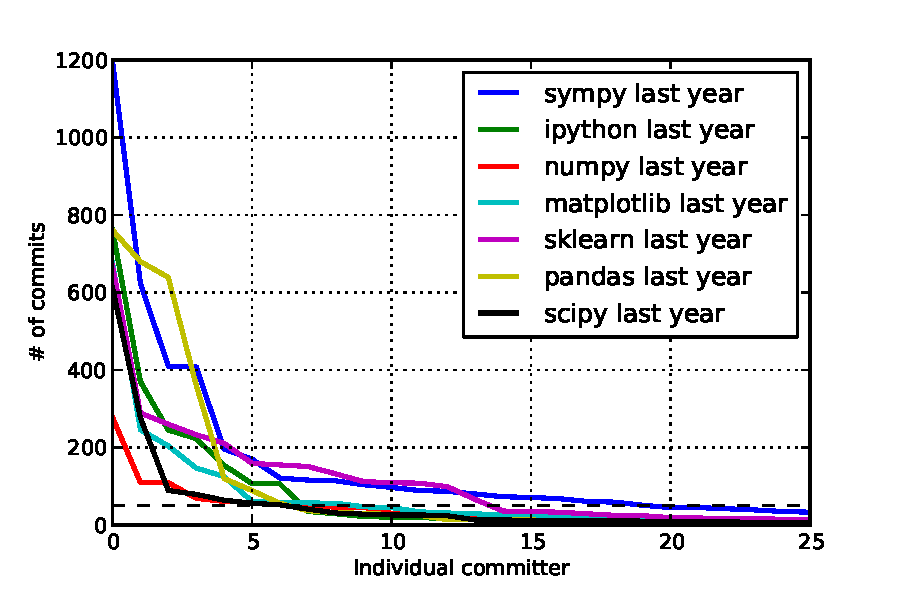
\includegraphics[width=4in]{commits1.pdf}
%%   \end{block}
%% \end{frame}
%%
%% \begin{frame}{Git Commit Plots}
%%   \begin{block}{Last Year}
%%     \begin{itemize}
%%     \item The dotted line is 50 commits.
%%     \item Rough measurement of each project's ``bus factor''
%%     \end{itemize}
%%   \end{block}
%% \end{frame}
%%
%% \begin{frame}{Git Commits Plots}
%%   \begin{block}{All Time}
%%     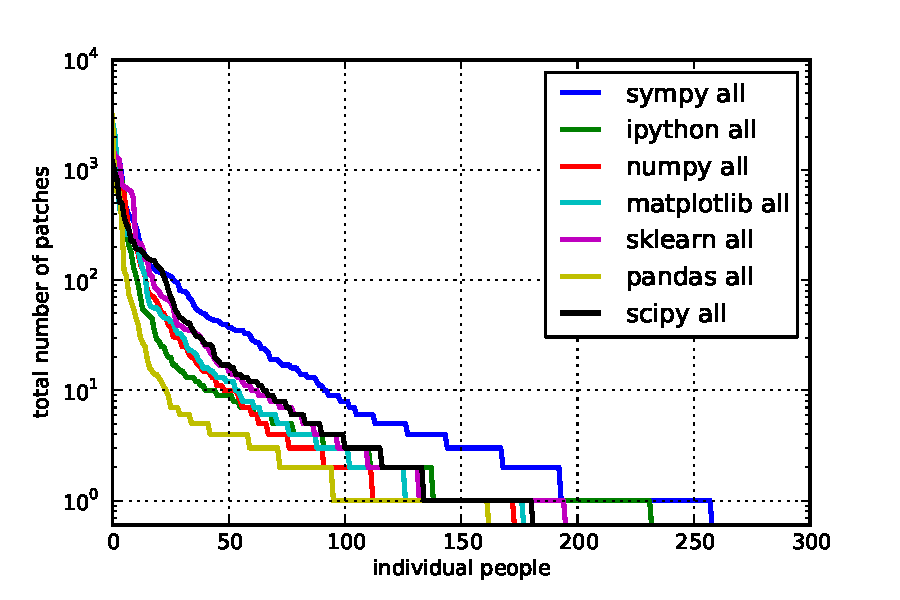
\includegraphics[width=4in]{commits-all.pdf}
%%   \end{block}
%% \end{frame}
%%
%% \begin{frame}{Git Commit Plots}
%%   \begin{block}{All Time}
%%     \begin{itemize}
%%     \item SymPy has more total contributors\footnote{some of the other projects are actually exaggerated,
%%         because they don't use \texttt{.mailmap}}
%%     \item SymPy has a very welcome and friendly community, which is open, and
%%       actively encourages contributions.
%%     \item The SymPy code base is very approachable to new contributors.
%%     \item To be fair, Google Code-In accounts for a lot of this\ldots
%%     \end{itemize}
%%   \end{block}
%% \end{frame}

\begin{frame}{Authors}
  \begin{multicols}{5}
    \tiny
        Chris Smith\\
        Aaron Meurer\\
        Mateusz Paprocki\\
        Ondřej Čertík\\
        Matthew Rocklin\\
        Julien Rioux\\
        Sergey B Kirpichev\\
        Raoul Bourquin\\
        Ronan Lamy\\
        Kirill Smelkov\\
        Øyvind Jensen\\
        Tom Bachmann\\
        Mario Pernici\\
        Sergiu Ivanov\\
        Saptarshi Mandal\\
        Thilina Rathnayake\\
        Stefan Krastanov\\
        Sean Vig\\
        David Li\\
        Rick Muller\\
        Brian E. Granger\\
        Vinzent Steinberg\\
        Gilbert Gede\\
        Vladimir Perić\\
        Raymond Wong\\
        Sachin Joglekar\\
        Fredrik Johansson\\
        Fabian Pedregosa\\
        Bharath M R\\
        Timothy Reluga\\
        Addison Cugini\\
        Thomas Hisch\\
        Jason Moore\\
        Manoj Kumar\\
        Guru Devanla\\
        Alexey U. Gudchenko\\
        hm\\
        Priit Laes\\
        Prasoon Shukla\\
        Matt Habel\\
        Francesco Bonazzi\\
        Alan Bromborsky\\
        Kundan Kumar\\
        Sudhanshu Mishra\\
        Tomo Lazovich\\
        Matt Curry\\
        Mary Clark\\
        Pablo Puente\\
        Jason Gedge\\
        Christopher Dembia\\
        Katja Sophie Hotz\\
        Aleksandar Makelov\\
        Ramana Venkata\\
        Brian Jorgensen\\
        Robert Johansson\\
        Kendhia\\
        Björn Dahlgren\\
        Joachim Durchholz\\
        Andy R. Terrel\\
        Grzegorz Świrski\\
        Sebastian Krämer\\
        Pearu Peterson\\
        Anurag Sharma\\
        Toon Verstraelen\\
        Joan Creus\\
        Siddhanathan Shanmugam\\
        Cristóvão Sousa\\
        Jorn Baayen\\
        Christian Muise\\
        Jeremias Yehdegho\\
        Matthew Hoff\\
        Kevin Hunter\\
        Riccardo Gori\\
        Alexander Hirzel\\
        Steve Anton\\
        Sanket Agarwal\\
        rathmann\\
        Robert Schwarz\\
        David Ju\\
        Angadh Nanjangud\\
        Luke Peterson\\
        Sahil Shekhawat\\
        Stephen Loo\\
        Harsh Gupta\\
        Yuriy Demidov\\
        Oliver Lee\\
        Comer Duncan\\
        Renato Coutinho\\
        Stepan Roucka\\
        Bilal Akhtar\\
        Miha Marolt\\
        Chetna Gupta\\
        Shipra Banga\\
        Randy Heydon\\
        Saurabh Jha\\
        Nathan Alison\\
        Niklas Thörne\\
        jerryma1121\\
        Sachin Irukula\\
        Sam Sleight\\
  \end{multicols}
\end{frame}

\begin{frame}{Authors (continued)}
  \begin{multicols}{5}
    \tiny

        Amit Saha\\
        Alkiviadis G. Akritas\\
        Akshay\\
        Brian Stephanik\\
        Robert Kern\\
        Angus Griffith\\
        Avichal Dayal\\
        Jim Crist\\
        Patrick Lacasse\\
        Swapnil Agarwal\\
        Gary Kerr\\
        Nicolas Pourcelot\\
        Natalia Nawara\\
        Mike Boyle\\
        Sherjil Ozair\\
        Huijun Mai\\
        Ljubiša Moćić\\
        Prafullkumar P. Tale\\
        Jim Zhang\\
        Ankit Agrawal\\
        Marek Šuppa\\
        Mark Shoulson\\
        Soumya Dipta Biswas\\
        Freddie Witherden\\
        Roberto Nobrega\\
        Felix Kaiser\\
        David Joyner\\
        Saroj Adhikari\\
        Sean Ge\\
        Zamrath Nizam\\
        Friedrich Hagedorn\\
        Jaroslaw Tworek\\
        Lennart Fricke\\
        Eric Nelson\\
        CJ Carey\\
        Aditya Shah\\
        Yuri Karadzhov\\
        Alexey Subach\\
        Rishabh Dixit\\
        Ryan Krauss\\
        Rajat Aggarwal\\
        Christian Bühler\\
        Min Ragan-Kelley\\
        Ananya H\\
        Mark Dewing\\
        Raphael Michel\\
        Demian Wassermann\\
        Dammina Sahabandu\\
        Andreas Kloeckner\\
        Sam Magura\\
        carstimon\\
        Tim Swast\\
        Roland Puntaier\\
        Chancellor Arkantos\\
        Chris Wu\\
        Christophe Saint-Jean\\
        Davy Mao\\
        Tomasz Buchert\\
        Tobias Lenz\\
        Harold Erbin\\
        richierichrawr\\
        Tarun Gaba\\
        Khagesh Patel\\
        Manish Gill\\
        Matthew Brett\\
        Nichita Utiu\\
        Piotr Korgul\\
        Stas Kelvich\\
        Varun Joshi\\
        shashank-agg\\
        Nimish Telang\\
        Stefano Maggiolo\\
        Óscar Nájera\\
        Chris Conley\\
        Sebastian Kreft\\
        Jochen Voss\\
        Stefen Yin\\
        Florian Mickler\\
        Tiffany Zhu\\
        Zeel Shah\\
        Tristan Hume\\
        Ben Lucato\\
        Stefan van der Walt\\
        Pramod Ch\\
        Abderrahim Kitouni\\
        Alexandr Popov\\
        Rom le Clair\\
        David Roberts\\
        Imran Ahmed Manzoor\\
        Benjamin McDonald\\
        Barry Wardell\\
        Andrew Straw\\
        Luis Garcia\\
        Manoj Babu K.\\
        Luca Weihs\\
        Amit Jamadagni\\
        Shravas K Rao\\
        Martin Povišer\\
        Julio Idichekop Filho\\
        Ted Horst\\
  \end{multicols}
\end{frame}

\begin{frame}{Authors (continued)}
  \begin{multicols}{5}
    \tiny

        Jens H. Nielsen\\
        Raffaele De Feo\\
        Heiner Kirchhoffer\\
        George Waksman\\
        Geoffry Song\\
        Emma Hogan\\
        Edward\\
        Tuomas Airaksinen\\
        Akshit Agarwal\\
        Nikolay Lazarov\\
        Akshay Srinivasan\\
        Venkatesh Halli\\
        Case Van Horsen\\
        Buck Shlegeris\\
        Pan Peng\\
        Bill Flynn\\
        Thomas Dixon\\
        Arpit Goyal\\
        Ashwini Oruganti\\
        Ben Goodrich\\
        Boris Timokhin\\
        Bradley Froehle\\
        Colleen Lee\\
        David Marek\\
        Dmitry Batkovich\\
        Fernando Perez\\
        Goutham Lakshminarayan\\
        Henrik Johansson\\
        Henry Gebhardt\\
        Jack McCaffery\\
        James Aspnes\\
        James Fiedler\\
        Jezreel Ng\\
        Juan Luis Cano Rodríguez\\
        Jurjen N.E. Bos\\
        Kalevi Suominen\\
        Kunal Arora\\
        Maciej Baranski\\
        Michael Mayorov\\
        Nikhil Sarda\\
        Oleksandr Gituliar\\
        Oscar Benjamin\\
        Patrick Poitras\\
        Pavel Fedotov\\
        Pradyumna\\
        QuaBoo\\
        Rajath S\\
        Sai Nikhil\\
        Sushant Hiray\\
        Thomas Wiecki\\
        Tomáš Bambas\\
        tsmars15\\
        Rizgar Mella\\
        Sambuddha Basu\\
        Puneeth Chaganti\\
        Prateek Papriwal\\
        Pierre Haessig\\
        Pauli Virtanen\\
        Paul Strickland\\
        Paul Scott\\
        Sebastian Krause\\
        Or Dvory\\
        Nicholas J.S. Kinar\\
        Max Hutchinson\\
        Matthias Toews\\
        Seshagiri Prabhu\\
        Shai 'Deshe' Wyborski\\
        Matthew Tadd\\
        Matt Rajca\\
        Markus Müller\\
        Shruti Mangipudi\\
        Shukla\\
        Marcin Kostrzewa\\
        Siddhant Jain\\
        Madeleine Ball\\
        Srinivas Vasudevan\\
        Lars Buitinck\\
        Konrad Meyer\\
        Kibeom Kim\\
        Kevin Goodsell\\
        Kazuo Thow\\
        Kaushik Varanasi\\
        Stepan Simsa\\
        Kaifeng Zhu\\
        Joseph Dougherty\\
        Jorge E. Cardona\\
        vishal\\
        Jonathan Miller\\
        Takafumi Arakaki\\
        Tarang Patel\\
        John Connor\\
        Johann Cohen-Tanugi\\
        Jeremy\\
        James Pearson\\
        James Goppert\\
        Thomas Sidoti\\
        Alexander Eberspächer\\
        James Abbatiello\\
        Tim Lahey\\
        Hubert Tsang\\
  \end{multicols}
\end{frame}

\begin{frame}{Authors (continued)}
  \begin{multicols}{5}
    \tiny

        Gregory Ksionda\\
        Gert-Ludwig Ingold\\
        Fawaz Alazemi\\
        Faisal Anees\\
        Erik Welch\\
        Abhinav Chanda\\
        Elrond der Elbenfuerst\\
        Eh Tan\\
        Dhruvesh Vijay Parikh\\
        Tyler Pirtle\\
        David Lawrence\\
        Vasily Povalyaev\\
        Christian Schubert\\
        Vinay Kumar\\
        Vinit Ravishankar\\
        Carsten Knoll\\
        Vlad Seghete\\
        Vladimir Lagunov\\
        Bernhard R. Link\\
        Benjamin Gudehus\\
        Benjamin Fishbein\\
        Bastian Weber\\
        Andrew Docherty\\
        Andrej Tokarčík\\
        Andre de Fortier Smit\\
        Anatolii Koval\\
        marshall2389\\
        Ambar Mehrotra\\
        Ali Raza Syed\\
        sevaader\\
        Alexandr Gudulin\\
        Roberto Colistete, Jr.\\
        Robert Cimrman\\
        Robert\\
        Łukasz Pankowski\\
        Ralph Bean\\
  \end{multicols}
\end{frame}

\begin{frame}{Here at SciPy}
  \begin{block}{Talks}
    \begin{itemize}
    \item \normalsize Jason Moore, \textit{Multibody Dynamics and Control with Python}
      (Tutorial). \\ \footnotesize Monday 8:00 AM - 12:00 PM - Rm 105
    \item \normalsize Matthew Rocklin, \textit{Taking Control - Enabling Mathematicians and Scientists}. \\ \footnotesize Tuesday 2:15
      PM - 2:45 PM - Grand Ballroom
    \item \normalsize Matthew Rocklin, \textit{Blaze: Building a Foundation
      for Array-Oriented Computing in Python}. \\ \footnotesize Thursday 11:15
      - 11:45 - Rm 204
    \item \normalsize Aaron Meurer, \textit{Conda: a Cross-Platform Package Manager for Any Binary Distribution}. \\
      \footnotesize Wednesday 11:45 AM - 12:15 PM - Rm 204
    \end{itemize}
  \end{block}
\end{frame}

\begin{frame}{Here at SciPy}
  \begin{block}{Bof}
    \begin{itemize}
      \item SymPy BoF - Wednesday 5:30 PM - 6:30 PM - Rm 203
    \end{itemize}
  \end{block}
  \begin{block}{Sprints}
    Come sprint with us!
    \begin{itemize}
    \item Releasing SymPy 0.7.6
    \item Assumptions
    \item Whatever interests you
    \item Lot's of tasks that are easy for new contributors
    \item Friday and Saturday
    \end{itemize}
  \end{block}
\end{frame}

\begin{frame}
\Huge Let's begin!
\end{frame}
\end{document}
